\begin{frame}{Implementations}
    \begin{itemize}
      \item LR: Logistic Regression
      \item LDA: Linear Discriminant Analysis
      \item KNN: K-Neighbors Classifier
      \item CART: Decision Tree Classifier
      \item NB: GaussianNB
      \item SVM: SVC
    \end{itemize}

    \begin{minipage}{0.5\textwidth}
        \centering
        \begin{figure}
    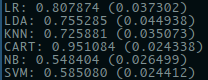
\includegraphics[width=.9\linewidth]{featureless1.png}
        \caption{Featureless}
        \end{figure}
    \end{minipage}%
    \begin{minipage}{0.5\textwidth}
        \begin{figure}
        \centering
    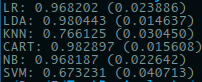
\includegraphics[width=.9\linewidth]{feature1.png}
        \caption{Feature}
        \end{figure}
    \end{minipage}
\end{frame}


\begin{frame}{Feature Implementation}
    Manual Feature Selection:
    \begin{itemize}
        \item Command length
        \item Proportion of Upper case
        \item Proportion of Special characters ('"\#\$\%\&\textbackslash ()*+-/:;=!?@\{\})
        \item Proportion of '
        \item Proportion of $\vert$
        \item Proportion of \^{}
        \item Number of 'cmd' and 'power' strings
        \item Presence of '-f' or '-F' strings
    \end{itemize}
\end{frame}


\begin{frame}{Models Evaluation}
    \begin{figure}
    \centering
    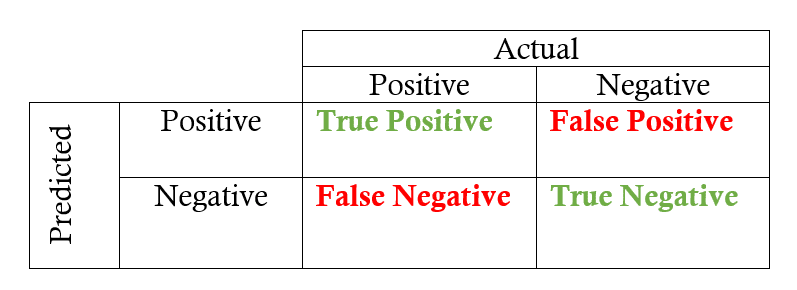
\includegraphics[width=.6\linewidth]{tpfp.png}
    \caption{True/False Positvie/Negative}
    \end{figure}

    \begin{figure}
    \centering
    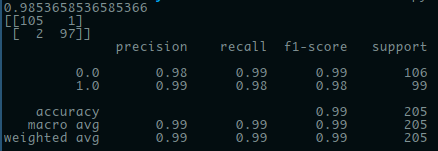
\includegraphics[width=.9\linewidth]{lda_eval1.png}
    \caption{LDA Evaluation}
    \end{figure}
\end{frame}

\begin{frame}{Demo}
\end{frame}




\begin{frame}{Future Work}
    \begin{itemize}
        \item Evaluate more models
        \begin{itemize}
            \item And more detailed testing (training time, ...)
        \end{itemize}
        \item Look into Feature selection
        \begin{itemize}
            \item Auto selection
            \item Importance Evaluation
        \end{itemize}
        \item Look into Dataset
        \begin{itemize}
            \item More obfuscation methods?
        \end{itemize}
        \item Creative Solutions to the Problem
        \item Get more detailed project's specifications 
    \end{itemize}
\end{frame}
